\documentclass[conference]{IEEEtran}

\ifCLASSINFOpdf
\else
\usepackage[dvips]{graphicx}
\fi

\usepackage{epsfig}
\usepackage{graphics}
\usepackage{graphicx}

\usepackage[cmex10]{amsmath}

\usepackage{flushend}


%\hyphenation{op-tical net-works semi-conduc-tor}


\begin{document}

\title{Mechanistic modeling of collective vehicular dynamics reproduces empirical features of urban traffic}

\author{\IEEEauthorblockN{R. Alfred Ajay Aureate and Sitabhra Sinha}
\IEEEauthorblockA{The Institute of Mathematical Sciences,\\
CIT Campus, Taramani, Chennai 600113, India\\
Email: alfredajay@imsc.res.in, sitabhra@imsc.res.in}}

\maketitle

%=============================================================================%

\begin{abstract}
Despite the recent surge of interest in studying various aspects of
traffic dynamics, congestion behavior in urban road networks (which is
characterized by extremely high vehicular densities and a large number
of intersections often controlled by signals) is not
yet well-understood.  In this article, we have presented a
mechanistic model for reproducing large-scale collective features of
congestion behavior from
the microscopic dynamics of individual vehicles interacting with each
other. By employing a detailed Newtonian description of the
time-evolution of velocity and acceleration of each vehicle, and
coupling it with a kinetic Monte Carlo simulation approach introduced
by us earlier,
we have presented an efficient modeling platform for investigating
macroscopic patterns of urban
congestion. In contrast to discrete cellular automata
models of traffic flow, our continuous-time, continuous-space modeling
of traffic flow in the presence of stochastic fluctuations 
approaches closer to reality. We have obtained fundamental diagram of
simulated urban traffic in the presence of a signal. The flow appears
to be relatively constant over a broad range of traffic densities
indicating that the traffic signal plays an important role in
smoothing out variations in traffic flow
that may result from fluctuations in the vehicle movements. 
We have also reproduced the empirically observed power-law scaling in
the distributions of congestion times. Our results underline the
important role played by the heterogeneity in the characteristics of
individual vehicles in producing long periods of congestion in urban
settings.
\end{abstract}

\IEEEpeerreviewmaketitle

%=============================================================================%

\section{Introduction}

%%%%%%%%%%%%%
As a result of advances in computer hardware and simulation
techniques, it is now possible to model large-scale social dynamics
involving interactions between a large number of
autonomous agents. The aim of such models is to understand macroscopic
phenomena that is observed at the level of the system or the
collective as an emergent phenomena, arising self-organizedly 
from the micro-dynamics of individual constituents~\cite{Ball2003}.
One of the most striking examples of such phenomena is the 
transition from free flowing traffic to a
jammed state and vice versa when the density of vehicles on a road is
altered~\cite{Helbing2001,Chakrabarti2007}.
Although the dynamics of vehicular traffic has been studied for
decades using fluid dynamical models, the introduction of
discrete cellular automata models by Nagel and Schreckenberg to study
highway traffic~\cite{Nagel1992} has resulted in a surge of interest
in describing complex patterns of collective vehicular movement 
using simple microscopic models. While this has resulted in a deeper
understanding of freeway traffic dynamics, the situation in an urban
setting,
marked by relatively high vehicular densities and the presence of
signals that coordinate movement of cross-flowing traffic traveling
along several directions, is not yet as well explicated.

Studying urban traffic congestion is extremely significant both in
terms of scientific and economic perspective, as a better
understanding of how jams occur and the duration for which they
persist can help in building more efficient transport infrastructures
in cities. Also, as first reported in Ref.~\cite{Majith2015}, the
congestion times, i.e., the duration for which a vehicle moves with a
speed less than a specified value, follows a heavy-tailed distribution
typically described by a power law. This is in stark contrast to an
exponential nature for the distribution which is expected in general
for a memory-less random process, with the random nature arising from
the existence of a large number of independent
components. Thus, the existence
of non-trivial macroscopic phenomena arising from urban traffic
dynamics makes it of great scientific importance also.

By studying the factors that affect traffic congestion, one
would be able to deduce aspects which are crucial for the control of
urban traffic and for reducing congestion.
We have previously proposed a microscopic model of vehicular dynamics
that uses a kinetic Monte-Carlo simulation approach~\cite{Majith2016}
that can reproduce the power-law characteristics of the distribution
of waiting times. However, there was a phenomenological element in the
model specifically in the way heterogeneity is introduced in the
response of vehicles to the space available in front of them on a road
(the headway distance). As such heterogeneity is crucial for
generating the heavy-tailed nature of the congestion time
distribution, we have in this article proposed a new mechanistic model
that uses a Newtonian description of the movements of each vehicle to
provide a more complete description. It is able to represent reality
more accurately and allows us to identify which aspects of vehicular
heterogeneity plays an important role in governing the exponents of the
power-law tails that characterize the nature of the distributions of
congestion times. In particular, apart from reproducing such macroscopic
features, the model also produces micro-dynamics of individual
vehicles that are a closer approximation to reality, e.g., the speed
and acceleration time-profiles of actual taxis traveling in major
Indian metropolises (Fig.~\ref{taxi_acc}).

\begin{figure}
%    \centering
{    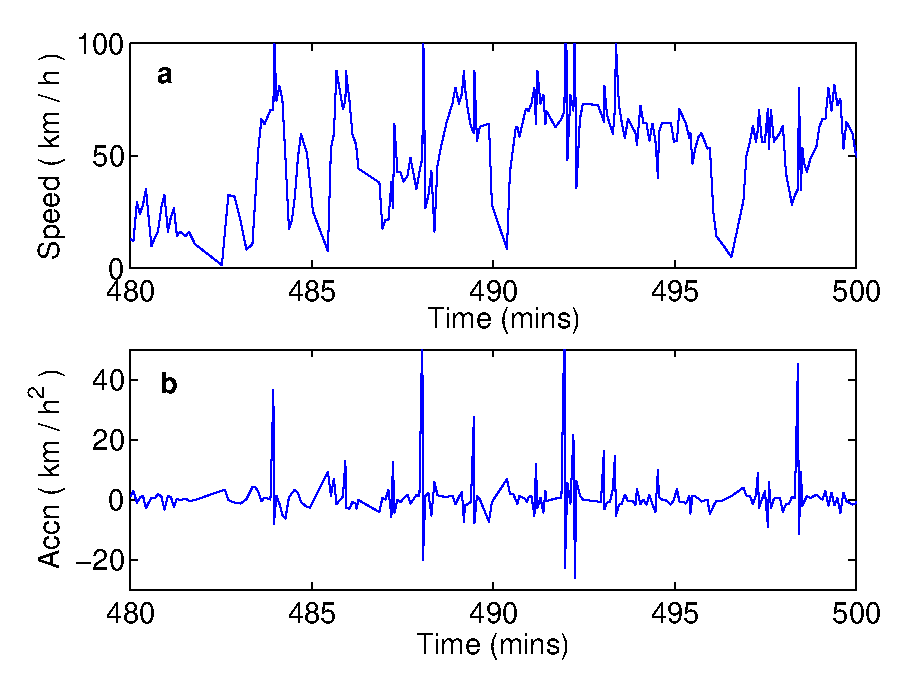
\includegraphics[width=9.0cm, angle=0]{figures/fig1.eps}}
\caption{Time evolution of (a) speed and (b) acceleration of a
particular vehicle in New Delhi recorded from GPS trace data during 
the period 1:30 pm - 1:50 pm (IST) on Jan 10, 2013 obtained from {\em
Traffline}~\cite{traffline}.}
    \label{taxi_acc}
\end{figure}

%=============================================================================%

\section{Model}
%Bass model
In the kinetic Monte Carlo model that had been introduced earlier in Ref.~\cite{Majith2016}, the velocities are abruptly changed every time step (depending on the headway distance) which is not the case in real life as the empirical data suggests in Fig.~\ref{taxi_acc}. Instead, the control mechanisms are in fact acceleration based in reality, namely - accelerator or brake. So, in this paper we intend to improvise the velocity-based model to incorporate the acceleration-based controls and effects. Moreover, the earlier model was phenomenological, whereas this one is more mechanistic in approach. % This would in turn smoothen out the velocity vs time plot as expected from the empirical data.

Similar to the model in Ref.~\cite{Majith2016}, here too we assume a single lane with fixed number of vehicles moving only in one direction. %In order to avoid boundary issues, a circular road is considered.
To ensure that constant traffic density is maintained without running into problems due to the  adjusting of the input and output rates, we assume periodic boundary conditions for the single lane or in simpler terms, a circular road. Also, the vehicles are externally controlled by a signal which is placed at one end of the road. %This signal basically represents the cross-over traffic.
The signal controls cross traffic at an intersection (signal controlled characterizes urban traffic). Now, instead of just updating the velocities of each vehicle at every instant, we update acceleration as follows:

\begin{equation}
\begin{split}
    \frac{dx_{i}}{dt} &= v_{i}\\
    \frac{dv_{i}}{dt} &= -(\gamma_{i} + \xi(x,t))v_{i} + \beta_{i}\bigg(\frac{d_{i}-v^{rel}_{i}\tau_{i}}{d_{i}+1}\bigg)
\end{split}
\label{dxdv}\end{equation}

where,

% not sure if we can use $\gamma(1+\epsilon\xi(x.t))$

$\gamma_{i}$ : drag rate due to friction of the road surface for car $i$.

$\xi$ : space and time dependent perturbation ( $>0$ ) in the drag rate that affects just a random car for each time step, representing possibly a pothole or applying of brake, etc.

$\beta_{i}$ : maximum acceleration possible (by stepping on %or applying
the accelerator).

$\tau_{i}$ : reaction time of the car-driver interface of car $i$.

$d_{i}$ : headway distance available in front of car $i$ to move without colliding. $d_{i}=|x_{i+1}-x_{i}|$, where $x_{i+1}$ and $x_{i}$ are positions of cars $i+1$ and $i$, respectively.

$v^{rel}_{i}$ : relative velocity of the car in front with respect to the car under consideration ($i$). $v^{rel}_{i}=v_{i+1}-v_{i}$.

Maximum velocity could then be given by, $v^{max}_{i}=\beta_{i}/\gamma_{i}$ (for a single car in an otherwise empty road $\frac{dv_{i}}{dt}=-\gamma_{i} v_{i} + \beta_{i}$)


\begin{figure}
%    \centering
{    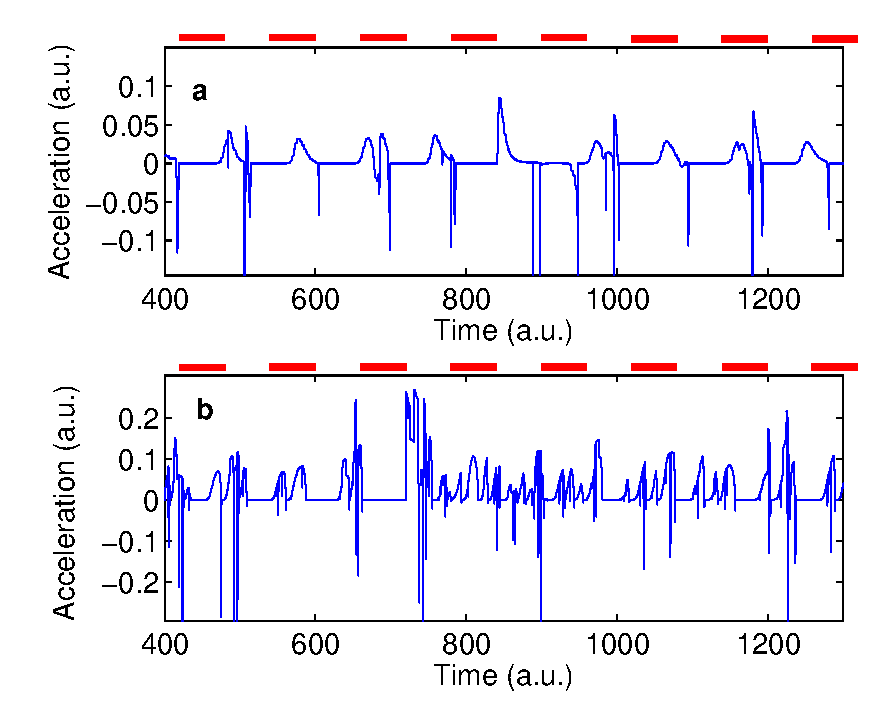
\includegraphics[width=9.0cm, angle=0]{figures/fig2_v2.eps}}
\caption{Time-evolution of acceleration for an individual 
vehicle from a simulation of the model described in the text with $N =
100$ vehicles. Panel (a) shows the homogeneous
situation where all vehicles are identical while in panel (b) the 
heterogeneous situation where
the vehicles have distinct characteristics (randomly chosen from 
distributions with specified means) is shown.
For (a) all the cars have $\gamma=0.2$, $\beta=0.2$ and $\tau=0.3$.
For (b) the mean values of the parameters (averaged over all vehicles 
in the simulation) are
$\langle \gamma \rangle =0.02$, $\langle \beta \rangle =0.2$ and
$\langle \tau \rangle =0.03$. In both cases the noise $\xi$ is chosen
from a uniform distribution over $[0.0.6]$. The periods during which
the
signal is red is indicated with color red horizontal bars shown along
the top of the figure.}
%    \caption{Variation of acceleration over time from the simulation. The traffic signal is marked with red. a) shows the variation of the instantaneous acceleration for a single car when we assume all identical cars with identical parameter values. b) similarly shows the variation of instantaneous acceleration when the parameter values for each car is different from each other.}
    \label{acc_t}
\end{figure}


In all the figures, except figure \ref{taxi_acc}, we either choose identical values of $\gamma$, $\beta$ and $\tau$ or random values for each car at the beginning of each simulation.%values remain the same though throughout the simulation
Without loss of generality, for each car, we pick those three parameter values from a corresponding gamma distribution. We chose gamma distribution so that we could analyze from a range of distributions by changing just one parameter (the shape parameter). By averaging over several such realizations the probability distribution of the waiting time is calculated. This exercise would therefore provide an insight as to which (inherent) characteristic of the car-driver-road system is crucial for the power-law behavior of the waiting time. It has already been shown that the power-law could emerge just from simple dynamics, without even considering any network structure nor multi-lanes, in Ref.~\cite{Majith2016}. However, the influence of external characteristics like the signal cycle, traffic density and duty ratio (of the signals), over the power-law behavior will be published elsewhere.

The first term in the acceleration Eqn. (\ref{dxdv}) represents the friction due to the road surface and it is proportional to the instantaneous velocity. Similarly, the second term represents the acceleration applied by the driver at every time step. It is directly proportional to the headway distance available in front for the vehicle to move. We have used an hyperbolic functional form to represent the dependence of the applied acceleration on the headway distance, just to ensure that the applied acceleration saturates to a maximum value $\beta$ as the headway distance increases. We have also taken into account the time-lag taken by the car-driver system to respond. So, the actual headway distance ($d-v^{rel}\tau$) would be lower than the physical headway distance, $d$. %Since $d\gg v_{rel}\tau$ usually,
%\[\frac{d_{i}-v^{rel}_{i}\tau_{i}}{d_{i}-v^{rel}_{i}\tau_{i}+1}\approx \frac{d_{i}-v^{rel}_{i}\tau_{i}}{d_{i}+1}\]




\begin{figure}
%    \centering
{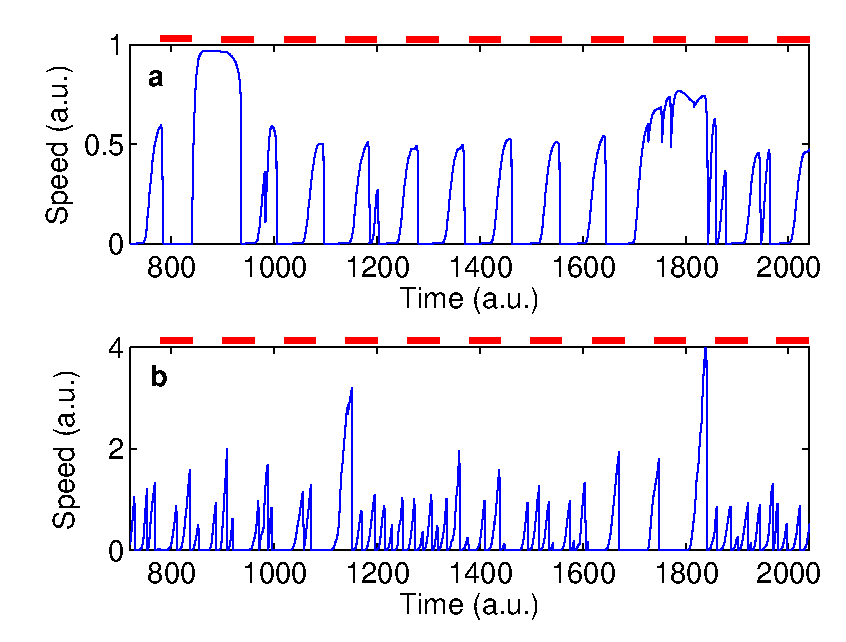
\includegraphics[width=9.0cm, angle=0]{figures/fig3_v4.eps}}
\caption{Time evolution of velocity for an individual
vehicle from a simulation of the model described in the text with $N =
100$ vehicles. Panel (a) shows the homogeneous
situation where all vehicles are identical while in panel (b) the
heterogeneous situation where
the vehicles have distinct characteristics (randomly chosen from
distributions with specified means) is shown.
For (a) all the cars have $\gamma=0.2$, $\beta=0.2$ and $\tau=0.3$.
For (b) the mean values of the parameters (averaged over all vehicles
in the simulation) are
$\langle \gamma \rangle =0.02$, $\langle \beta \rangle =0.2$ and
$\langle \tau \rangle =0.03$. In both cases the noise $\xi$ is chosen
from a uniform distribution over $[0.0.6]$. The periods during which the
signal is red is indicated with color red horizontal bars shown along
the top of the figure.}
%(c) The complementary cumulative probability
%distribution of speed of vehicles when they are a specific headway
%distance from the preceding vehicle (shown for four different values)
%exhibits an exponential behavior. (d) The mean velocity as a function
%of the headway distance $d$ shows a sigmoidal nature. The broken curve
%is a theoretical fit to the simulated data shown using circles.}

%    \caption{Variation of velocity over time in the simulation. Blue line shows the instantaneous velocity of a single car, whereas the dotted green line represents the instantaneous average velocity across the system. The swapping of the traffic signal is marked by red where marking over '1' represents the red signal and '0' represents green signal. a)  shows velocity variation over time when the cars are assumed to be 'identical' to each other, in the sense that the car-specific parameters are all same for each one of them. b) shows the velocity variation when the cars are assigned with different parameter values, namely $\gamma$, $\beta$ and $\tau$.}
    \label{vel_t}
\end{figure}



Based on the equations (\ref{dxdv}) for all cars, the subsequent time step $dt$ is calculated, for progressing time in the simulation based on two conditions: i) None of the cars are allowed to collide with the cars in front while the vehicles progress with constant acceleration during the time-step $dt$. ii) None of the cars' velocities are allowed to go below zero. The largest $dt$ value satisfying those conditions is chosen for updating the progression of time in the simulation. At time $n$ (using Newton's 2nd law we arrive at),

\begin{equation}
    dt_{n} = \min_{i}\left( \frac{-v_{i,n-1} + \sqrt{v_{i,n-1}^2 + 2a_{i,n-1}d_{i,n-1}}}{a_{i,n-1}}\right)
\end{equation}

where $v_{i,n-1}$ is the velocity, $a_{i,n-1}$ is the acceleration and $d_{i,n-1}$ is the headway distance at time $n$ for the car $i$. The $dt_{n}$ that is calculated here is now the time step chosen at time $n$. This adaptive selection of step-size allows us to mimic continuous-time, continuous-space dynamics more accurately. Note that the determinant (or the expression inside the square root) always remains non-negative as it is just the square of the final velocity (or the velocity attained just after the time step).

%=============================================================================%
\section{Results}
 %-----------------------------------------------------------------------------%

We have considered the vehicular density (i.e., the fraction of road
surface occupied by cars) to be $0.5$ in all cases reported here.
Also, the signal cycle runs for about 60 time units for each red and green
light. Given that, we observe from Fig.~\ref{acc_t}(a) that when the
cars and drivers are identical, the acceleration is a periodic
function that synchronizes closely with the signal cycle. On the other hand,
in Fig.~\ref{acc_t}(b) where the agents (car-driver systems) are assumed to be non-identical, the acceleration does not behave periodically, but rather in an erratic fashion. In fact, the maximum magnitude in both positive and negative directions has increased, which could possibly mean that the agents are applying stronger braking/acceleration because of the unpredictability. %quite behaving in an unpredictable and "aggressive" manner.




Such contrasting pattern in the acceleration gets smoothened out in
the velocity variation as time progresses, Fig.~\ref{vel_t}. Even
though the velocity variation in Fig.~\ref{vel_t}~(b) is more smooth
than the one with the stochastic noise in Ref.~\cite{Majith2016}, it still
has spikes and appears to be more unpredictable compared to
Fig.~\ref{vel_t}~(a). 
Again, because of higher maximum magnitudes for acceleration, we
observe higher maximum values of speed also in Fig.~\ref{vel_t}(b), even though overall average velocity of the system remains almost the same in both cases.


By comparing the Figs.~\ref{acc_t}(b) and \ref{vel_t}(b) with Figs.~\ref{taxi_acc}(b) and \ref{taxi_acc}(a) respectively, we could quite conclude that our model's prediction about the evolution of velocity or acceleration over time agrees well with the empirical data. One could notice the sudden "jerks" and prolonged calmness in the acceleration both in Figs.~\ref{taxi_acc}(b) and \ref{acc_t}(b). Similarly, one could also observe the spikes in the velocity profile in both Figs.~\ref{taxi_acc}(a) and \ref{vel_t}(b).

%Also, from the figure \ref{vel_t}(c) and (d), we notice that the
%exponential fluctuation for velocity and the sigmoidal relation
%between headway distance and velocity assumed in \cite{Majith2016} is
%satisfied by this model too, thereby making this model a more general
%one.


\begin{figure}
%    \centering
{    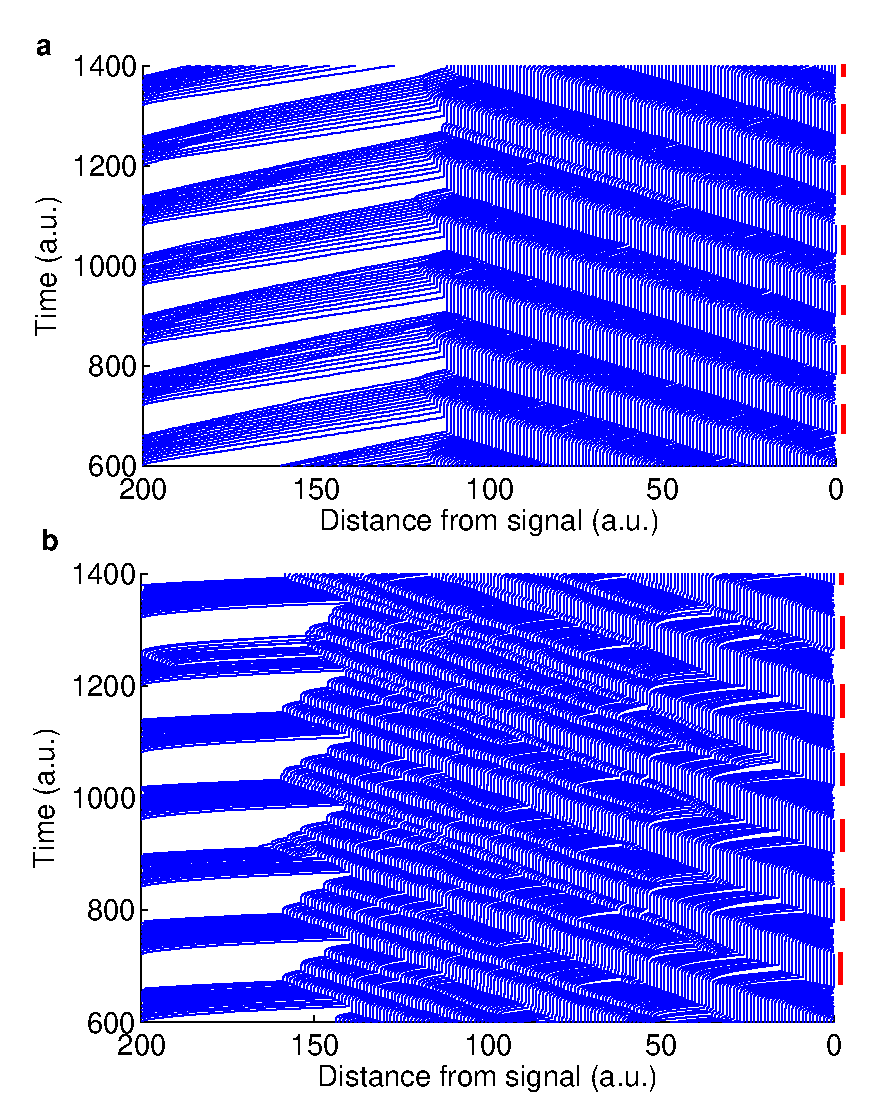
\includegraphics[width=9.0cm, angle=0]{figures/fig4.eps}}
\caption{Spatio-temporal evolution of simulated traffic showing trajectories
of individual vehicles with a signal located at the right end that
prevents vehicular movement at periodic intervals comparing the
homogeneous situation (a) where all cars are identical with the
heterogeneous case (b) where the cars have distinct (randomly chosen)
characteristics. The vehicular
density is (i.e., the fraction of road surface occupied by cars) is
$0.5$ in all cases. The ordinate indicates time so that when a vehicle
slows down the line becomes more vertical.
The red vertical bars at the right margin of the center and bottom
panels indicate when cars are not allowed to move past the signal
(the duration of the signal cycle is 120 a.u., with the light being
green and red for equal amounts of time).
}
%    \caption{Both the plots show the space-time evolution of all cars. Each line represents the space-time trajectory of a single car. Traffic signals are marked with red on the right side for reference. When we consider identical car-driver system (top), the space-time evolution of the cars kind of synchronize with each other and resembles very close to that of the deterministic case in \cite{Majith2016}, whereas we could observe (bottom) that there are various other perturbations causing an increase in the length of the jam when the car-driver systems are considered to be non-identical. Interestingly, unlike in the identical case (top), the non-identical nature of individuals (bottom) results in the reduction of the effect of any perturbation as it propagates backwards.}
    \label{spacetime}
\end{figure}



\begin{figure}
%    \centering
{    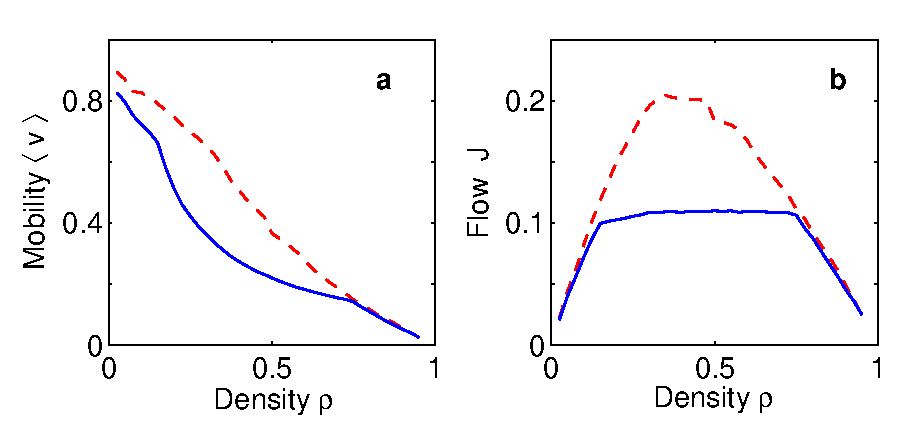
\includegraphics[width=9.0cm, angle=0]{figures/fig5.eps}}
\caption{The macroscopic fundamental diagrams representing the
traffic dynamics generated by the model presented here showing the
dependence of (a) mobility, i.e., average speed, and (b) flow, i.e.,
the average number of moving vehicle per unit time, on the vehicular density. 
The situation in the presence of a traffic signal with a signal cycle
of 120 time units (continuous curves) is compared with the diagram
obtained in the absence of any intersection or signal (broken
curves).}
    \label{fund}
\end{figure}



\begin{figure}
%    \centering
{    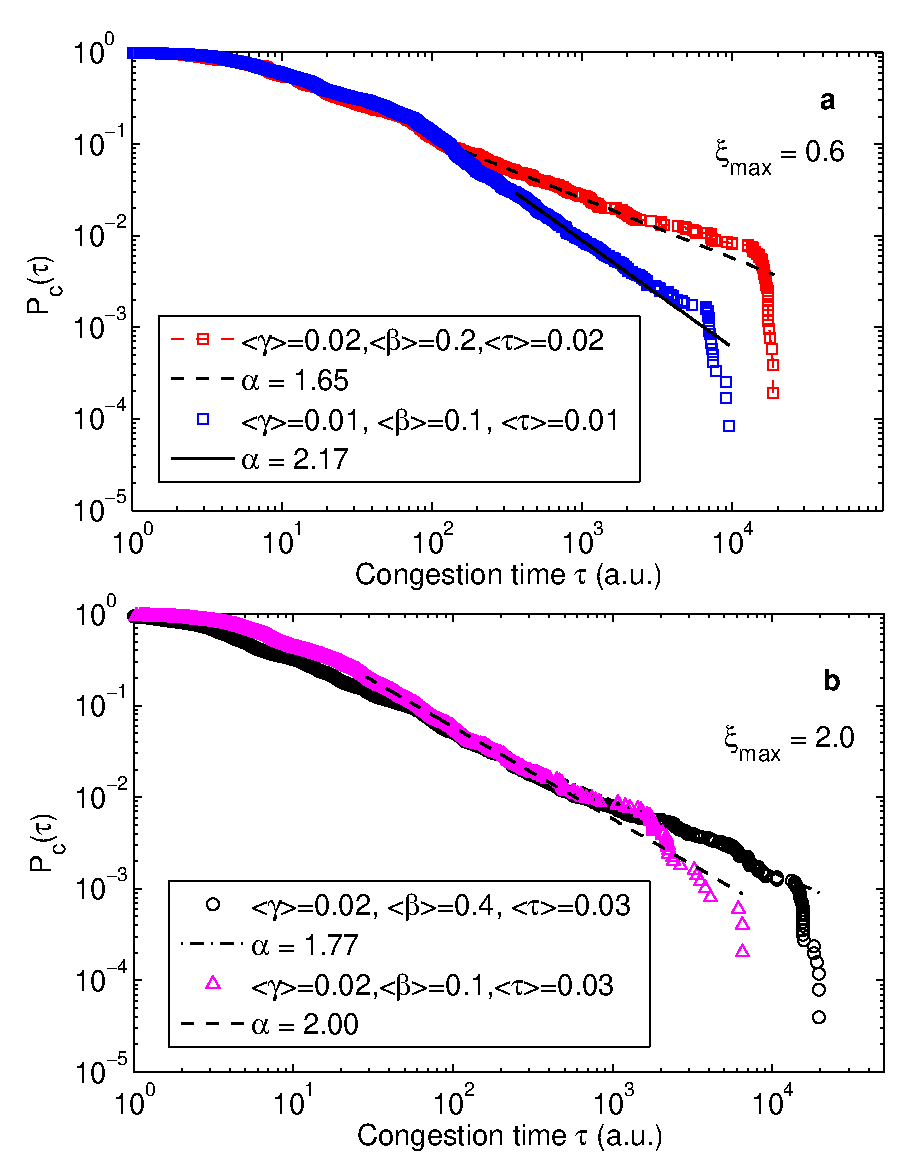
\includegraphics[width=9.0cm, angle=0]{figures/fig6.eps}}
\caption{The complementary cumulative probability distribution of the
congestion time $\tau$, i.e., the duration for which a vehicle moves
with a speed less than a specified value (threshold speed = $0.1$
a.u.),
shown for the model in the heterogeneous situation where all
vehicles have distinct characteristics. The mean values of the
parameters are for the different cases shown and are indicated in the
legend. The vehicles are subject to random noise $\xi$ in their deceleration
which is generated from a uniform distribution between $[0,
\xi_{max}]$. The two panels compare situations with (a) low and (b) high
levels of noise, $\xi_{max}$. The heavy-tailed nature of the
distributions have been fit to power-law forms, viz., 
$P_c(\tau) \sim
\tau^{(1-\alpha)}$
and 
the exponent values $\alpha$ for each of the curves are estimated 
using maximum likelihood technique.}
    \label{power_law_abt}
\end{figure}



\begin{figure}
%    \centering
{    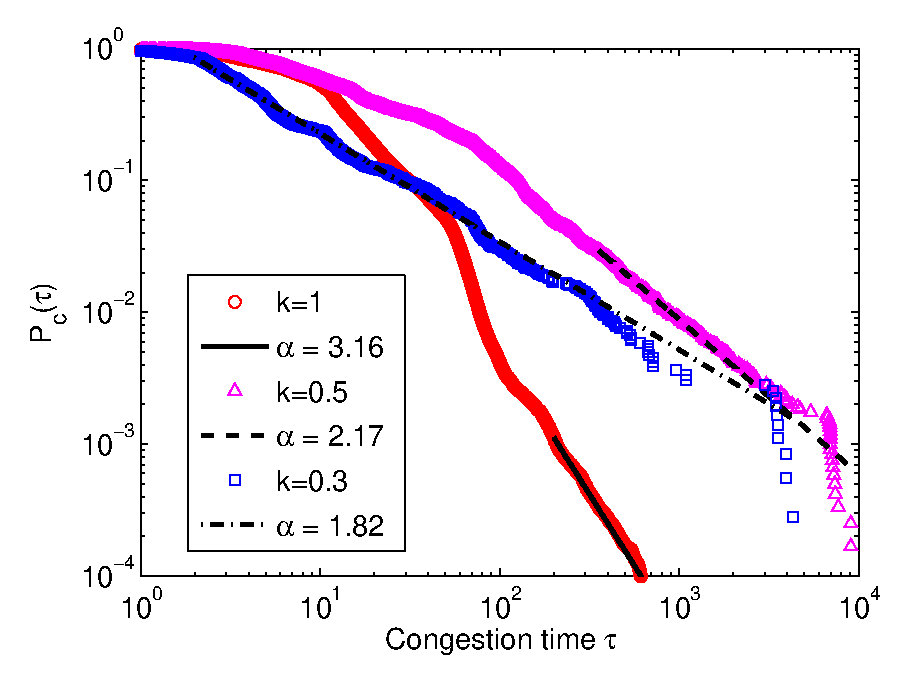
\includegraphics[width=9.0cm, angle=0]{figures/fig7.eps}}
\caption{The complementary cumulative distribution of the congestion
time $\tau$ for the model in the heterogeneous situation where all 
vehicles have distinct characteristics. The different curves
correspond to different types of heterogeneity for the distribution of
parameter values, obtained by varying the shape parameter $k$ of a
gamma distribution. In all other simulations shown here $k$ has been
chosen to be 0.5.}
    \label{power_law_gam}
\end{figure}



In Fig.~\ref{spacetime}, we plot the space-time trajectory of each car
as it moves along the single-lane road towards the signal (marked on
the right end). We notice from the plot on the top of
Fig.~\ref{spacetime} that the cars start behaving in a periodic and
deterministic fashion when the agents are assumed to be identical,
whereas there arises a lot of random perturbations in the trajectory
of the cars when the agents are assumed to be non-identical to each
other (bottom of Fig.~\ref{spacetime}). So, when the agents are non-identical, a lot of internal perturbations start arising, in addition to the effect of the signal. In the simulation, it has been made sure that the cars never collide at any instant, so we see that the trajectories never intersect nor touch each other. %Such constraint is ensured by picking the time step in such a way that the cars move with constant acceleration over the duration of that time step without colliding nor decreasing it's velocity below zero, meaning we assume that cars rather stop instead of moving in the reverse direction.




The fundamental diagram in Fig.~\ref{fund} shows how mobility $\langle v \rangle$ and flow $J$ varies as a function of density $\rho$.

Density here is defined as the number of cars per unit car length of the road, $\rho=\frac{P}{L}$, where $P$ is the number of cars and $L$ is the road length.

Mobility is given by,
\[\langle v \rangle = \frac{\text{Total distance travelled by all cars during simulation}}{(\text{Total duration of simulation})P}\]
and flow is $J=\langle v \rangle \rho$. The dotted red line shows how
the transition from free flow to jammed state occurs in an highway
(meaning in the absence of signals). From the blue line plot, we
observe that, unlike in an highway, this transition is not abrupt for the traffic flow with intersections (meaning with traffic signals). Instead, the flow, $J$ actually remains almost constant for a wide range of density values, causing a flattened plateau, Fig.~\ref{fund}(b). The mobility, on the other hand becomes more concave as a function of density, in the presence of traffic signals, Fig.~\ref{fund}(a).



We found using our mechanistic acceleration-based model, that the congestion times follow a power-law distribution, 
\begin{equation}
    P_c(\tau) \sim\tau^{(1-\alpha)}
\end{equation}

with varying exponent values $\alpha$ (where $\alpha$ is a
non-negative real number), as shown in Fig.~\ref{power_law_abt} and
Fig.~\ref{power_law_gam}. When the agents are assumed to be identical,
we have noticed from previous figures that the system very closely
resembles a deterministic one. So, we would only considered the
non-identical case here. As the values of $\xi$, $\langle \gamma
\rangle$, $\langle \beta\rangle$ and $\langle\tau \rangle$ are varied,
the power-law distribution of the congestion times has exponent very close to $1.6-2.2$. But, when we assume stochastic fluctuations in the
parameter values, meaning heterogeneity of the parameters $\gamma$,
$\beta$ and $\tau$, we then get a range of power-law exponents, from
$1.8-3.2$ for different choice of shape parameter of the gamma
distribution (especially for sub-exponential distributions), as shown
in Fig.~\ref{power_law_gam}. The exponent values of the power-law are obtained using the
Maximum-Likelihood method described in Clauset {\em et. al.} ~\cite{Clauset2009}. This provides a best power-law fit to the distribution that is obtained from the simulation.


\section{Conclusion}
In this report, we have presented a novel approach towards modelling the traffic congestion using a microscopic Monte-Carlo model. Following Newton's laws, with some fluctuations in terms of the non-identical nature of the car-driver system, we have shown that one could obtain waiting times following a power-law distribution. This therefore does not introduce any major fluctuations directly into the dynamics, as was done in Ref.~\cite{Majith2016}. Moreover, the range of exponent values, $\alpha$'s, agrees very well with the range of exponent values obtained from empirical data of various Indian urban metropolises, namely Bangalore, Bombay and New Delhi \cite{Majith2016},\cite{Majith2015}.

%=============================================================================%

\section*{Acknowledgments}

The authors would like to thank Krishna Jagannathan for help in
accessing the GPS trace data analyzed here, N. Abdul Majith for
initial work on mechanistic traffic modeling, Soumya Easwaran, Shakti
Menon and K Chandrashekar for assistance in data analysis, and IMSc (Institute of Mathematical Sciences)
for providing access to the high-performance computing facility.
This research was supported in part by the ITRA Media Lab Asia 
project ``De-congesting India's Transportation Network'' and IMSc
Complex Systems Project (XII Plan).

%=============================================================================%
%=============================================================================%

\begin{thebibliography}{1}
\bibitem{Ball2003}
{P.~Ball, ``The physical modelling of human social systems,'' {\em
Complexus}, vol. 1, pp.~190–206, 2003.}

\bibitem{Helbing2001}
{D.~Helbing, ``Traffic and related self-driven many-particle
systems,'' {\em Rev. Mod. Phys.}, vol. 73, pp.~1067-1141, 2001.}

\bibitem{Chakrabarti2007}
{B.~K.~Chakrabarti, A.~Chakraborti and A.~Chatterjee, Eds. ``
Econophysics and Sociophysics: Trends and perspectives''. 
{\em Weinheim: Wiley-VCH}, 2007.}

\bibitem{Nagel1992}
{K.~Nagel and M.~Schreckenberg, ``A cellular automaton model
for freeway traffic,'' {\em J. Phys. I}, vol. 2, pp.~2221–2230, 1992.}

\bibitem{Majith2015}
{N.~Abdul Majith and S.~Sinha, ``Statistics of stop-and-go traffic: Emergent properties of congestion 
behavior arising from collective vehicular dynamics in an urban environment,'' in {\em Proceedings of the 
7th International Conference on Communication Systems and Networks (COMSNETS)}, Bangalore, 2015, pp.~1-4.}

\bibitem{Majith2016}
{N.~Abdul Majith and S.~Sinha ``Dynamics of urban traffic congestion: A kinetic Monte Carlo
approach to simulating collective vehicular dynamics,'' in
{\em Proceedings of the
8th International Conference on Communication Systems and Networks
(COMSNETS)}, Bangalore, 2016, pp.~1-5.}

\bibitem{traffline}
http://www.traffline.com/

\bibitem{Clauset2009}
{A.~Clauset, C.~R.~Shalizi and M.~E.~J.~Newman, ``Power-law distributions 
in empirical data,'' {\em SIAM Review}, vol. 51, pp.~661-703, 2009.}

%\bibitem{PRL}
%{"Dynamics of traffic congestion" (to be published elsewhere)}

%\bibitem{Wheeler1989}
%{J.~A.~Wheeler, ``Information, physics, quantum: The search for
%links,'' in {\em Proceedings of the 3rd International Symposium on the
%Foundations of Quantum Mechanics}, Tokyo, 1989, pp.~354-368.}

%\bibitem{Zurek1990}
%{W.~H.~Zurek, Ed., {\em Complexity, Entropy, and Physics of
%Information}. New York: Addison-Wesley, 1990.}

%\bibitem{Sinha2006}
%{S.~Sinha, ``Phase transitions in the computational complexity of elementary
%cellular automata,'' in {\em Unifying Themes in Complex Systems},
%A.~A.~Minai and Y.~Bar-Yam, Eds. Berlin: Springer, 2006, 
%pp.~337-348.}

\end{thebibliography}

%=============================================================================%
%=============================================================================%

% that's all folks
\end{document}
